%  --------------------------------------------------------------------------
%  Semesterarbeit Single Sign-On Lösung für Django Dokumentation
%  Created by Marc Egli on 2012-04-02.
%  --------------------------------------------------------------------------

%  --------------------------------------------------------------------------
%  Latex Document Settings
%  --------------------------------------------------------------------------
\documentclass[
11pt, % Schriftgrösse
a4paper, % A4 Papier
BCOR10mm, % Absoluter Wert der Bindekorrektur, z.B. BCOR1cm
DIV14, % Satzspiegel festlegen siehe
       % http://www.ctex.org/documents/packages/nonstd/koma-script.pdf
footsepline = false, % Trennlinie zwischen Textkörper und Fußzeile
                     % bei normalen Seiten
headsepline, % Trennlinie zwischen Kopfzeile und Textkörper
             % bei normalen Seiten
oneside, % Zweiseitig
openright,
halfparskip, % Europäischer Satz mit Abstand zwischen den Absätzen
abstracton, % inkl. Abstract
listof=totocnumbered, % Abb.- und Tab.verzeichnis im Inhaltsverzeichnis
bibliography=totocnumbered % Lit.zeichnis in Inhaltsverzeichnis aufnehmen
]{scrreprt}

\usepackage[automark]{scrpage2} % Gestaltung von kopf- und Fußzeile
\usepackage[ngerman]{babel}
\usepackage[ngerman]{translator}
\usepackage{tocbasic}
\usepackage[utf8]{inputenc}
\usepackage{lmodern} % Latin Modern
\usepackage[T1]{fontenc}
\usepackage{hyphenat}
\usepackage{ae} % Schöne Schriften für PDF-Dateien
\usepackage{multirow} % tabellenzellen zusammenfassen
\usepackage{float}

% Tradmark
\def\TTra{\textsuperscript{\texttrademark}}

%1.5 Zeilenabstand
\usepackage[onehalfspacing]{setspace}

% Festlegung des Seitenstils (scrpage2)
\pagestyle{scrheadings}
\clearscrheadfoot
\automark[]{chapter}

% \lehead{\sffamily\upshape\headmark}
% \cehead{}
% \rehead{}
% \lefoot[\pagemark]{\upshape \pagemark}
% \cefoot{}
% \refoot{}
% \lohead{}
% \cohead{}
\lohead{\sffamily\upshape\headmark}
\lofoot{}
\cofoot{}
\rofoot[\pagemark]{\scshape \pagemark}

% Surround parts of graphics with box
\usepackage{boxedminipage}

% Package for including code in the document
\usepackage{listings}

% If you want to generate a toc for each chapter (use with book)
\usepackage{minitoc}
\usepackage{longtable}

% Abkürzungsverzeichnis erstellen.
\usepackage[printonlyused]{acronym}

% schöne Tabelle zeichnen
\usepackage{booktabs}
\renewcommand{\arraystretch}{1.4} %Die Zeilenabstände in Tabllen angepasst.

% für variable Breiten
\usepackage{tabularx}

% Durchgestrichener Text
\usepackage[normalem]{ulem} %emphasize weiterhin kursiv

% This is now the recommended way for checking for PDFLaTeX:
\usepackage{ifpdf}

\usepackage{eurosym}

\usepackage{natbib}

\usepackage{paralist}

\usepackage{array,ragged2e}

% glossary
\usepackage[toc,xindy,acronym, numberline]{glossaries}

\usepackage[]{hyperref}
\hypersetup{
  bookmarks=true,         % show bookmarks bar?
  unicode=true,           % non-Latin characters in Acrobat’s bookmarks
  pdftoolbar=true,        % show Acrobat’s toolbar?
  pdfmenubar=true,        % show Acrobat’s menu?
  pdffitwindow=true,      % window fit to page when opened
  pdfstartview={FitH},    % fits the width of the page to the window
  pdftitle={Semesterarbeit},   
  pdfauthor={Marc Egli},
  pdfsubject={Single Sign-On Lösung für Django},
  pdfcreator={TeX Live 2011},
  pdfproducer={pdfTeX, Version 3.1415926-2.3-1.40.12},
  pdfnewwindow=true,      % links in new window
  colorlinks=true,       % false: boxed links; true: colored links
  % linkcolor=blue,          % color of internal links
  % citecolor=black,        % color of links to bibliography
  % filecolor=magenta,      % color of file links
  % urlcolor=cyan          % color of external links
  linkcolor=black,          % color of internal links
  citecolor=black,        % color of links to bibliography
  filecolor=black,      % color of file links
  urlcolor=black          % color of external links
}

\ifpdf
    \usepackage[pdftex]{graphicx}
\else
    \usepackage{graphicx}
\fi

\makeatletter 
\let\orgdescriptionlabel\descriptionlabel 
\renewcommand*{\descriptionlabel}[1]{% 
  \let\orglabel\label 
  \let\label\@gobble 
  \phantomsection 
  \edef\@currentlabel{#1}% 
  %\edef\@currentlabelname{#1}% 
  \let\label\orglabel 
  \orgdescriptionlabel{#1}% 
} 
\makeatother 

%!TEX root = index.tex
\newglossaryentry{Git}
{
  name=Git,
  description={Ein Werkzeug mit welchem man Quellcode versionieren kann. \url{http://git-scm.com/}}
}

\newglossaryentry{OpenID-Provider}
{
  name=OpenID-Provider,
  description={Ein Dienst welcher seinen Benutzern je eine OpenID zur Verfügung stellt. Bekannte OpenID-Provider sind Google, Yahoo und flickr},
  plural=OpenID-Provider,
}

\newglossaryentry{OpenID-Relying-Party}
{
  name=OpenID-Relying-Party,
  description={Eine Applikation welches seinen Benutzern die Anmeldung mit
               einer OpenID ermöglicht},
  plural=OpenID-Relying-Parties 
}

\newglossaryentry{Autorisierung}
{
  name=Autorisierung,
  description={Synonym für Berechtigung oder Erlaubnis \footnote{\url{http://www.duden.de/rechtschreibung/Autorisierung}}}
}

\newglossaryentry{Authentifikation}
{
  name=Authentifikation,
  description={Identitätsprüfung eines Benutzers als Zugangs- und Rechtekontrolle für ein System (z. B. durch Passwort) \footnote{\url{http://www.duden.de/rechtschreibung/Authentifikation}}}
}

\newacronym{url}{URL}{Uniform resource locator}
\newacronym{api}{API}{Application Programming Interface}
\makeglossaries

%  --------------------------------------------------------------------------
%  Start Document
%  --------------------------------------------------------------------------
\title{Single Sign-On Lösung für Django}

\author{Semesterarbeit in Informatik\\
    \\
    Studierender - Marc Egli\\
	Auftraggeber - Silvan Spross\\
    Projektbetreuer - Lukas Eppler\\
	\\
	HSZ-T - Technische Hochschule Zürich}

\date{Februar 2012 bis Juli 2012}


\begin{document}
  \ifpdf
    \DeclareGraphicsExtensions{.pdf, .jpg, .tif}
  \else
    \DeclareGraphicsExtensions{.eps, .jpg}
  \fi
  
  \maketitle
  %!TEX root = ../index.tex
Diese Semesterarbeit widmet sich einem den meisten Webagenturen welche für ihre Kunden viele Webseiten betreuen, bekannten Problem: Zugangsdaten werden oftmals zentral und allen Mitarbeitern welche Zugang zu den Webseiten benötigen zugänglich abgelegt um den schnellen Zugriff auf Administrationsbereiche zu gewährleisten. Dies geschieht zum Wohle des Kunden und im Vertrauen darauf, dass alle Mitarbeiter mit guter Absicht handeln und auch nach dem Verlassen der Agentur nicht die Zugangsdaten die ihnen anvertraut wurden missbrauchen.

Als Ergebnis dieser Arbeit entstand ``django-admin-sso''. Es handelt sich dabei um eine Django Applikation welche Mitarbeiter über ein zentrales System autorisiert und dadurch eine Lösung für das zuvor erwähnte Problem bietet.


  \pagenumbering{Roman}
  
  \tableofcontents
  
  \chapter{Personalienblatt}
  %!TEX root = ../index.tex
\begin{tabbing}
\hspace*{4cm} \= \kill
Name, Vorname: \> {\bf Egli, Marc} \\
Adresse: \> {\bf Altstetterstrasse 257} \\
PLZ, Wohnort: \> {\bf 8048 Zürich} \\
\\
Geburtsdatum: \> {\bf 13.11.1983} \\
Heimatort: \> {\bf Winterthur} \\
\end{tabbing}
  
  \chapter{Bestätigung}
  %!TEX root = ../index.tex
Hiermit bestätige ich, Marc Egli, dass ich die vorliegende Semesterarbeit ``Single Sign-On Lösung für Django'' im Rahmen der geltenden Reglemente selbstständig erarbeitet habe.\\
\\
Zürich, den 17. Juli 2012\\
\\\\
Marc Egli

  
  \chapter{Einleitung}
  \label{cha:Einleitung}
  \pagenumbering{arabic}
  %!TEX root = ../index.tex
\section{Ausgangslage}
\label{sec:EinleitungAusgangslage}
Die Agentur allink.creative Betreibt für ihre Kunden diverse Django basierte 
Webapplikationen. Diese Applikationen besitzen jeweils einen 
Administrations-Bereich, in welchem man sich mit Benutzername und Passwort 
einloggen kann. Da allink.creative anfangs 2012 fast 100 solche 
Webapplikationen in Betrieb hat, werden die Login-Daten zum Teil mehrfach 
verwendet.

\section{Problemstellung}
\label{sec:Problemstellung}
Nicht alle verwendeten Login-Daten sind sauber dokumentiert. Darum muss man 
teilweise den Entwickler einer Applikation nach den Login-Daten fragen, oder 
die gängigsten Passwörter durchprobieren um Zugriff auf den 
Administrations-Bereich zu erhalten. Zudem gibt es keine Möglichkeit einem 
Mitarbeiter welcher die Agentur verlässt den Zugang zu Sperren, ohne dass man 
in sämtlichen Applikationen die Zugangsdaten ändert.

\section{Zielsetzung}
\label{sec:Zielsetzung}
Das Hauptziel dieser Arbeit besteht darin, den Zugang zu den Administrations-Bereichen über ein zentrales System zu Regeln.


  \chapter{Planung}
  \label{cha:Planung}
  %!TEX root = ../index.tex
Zu Beginn der Arbeit waren zwei Daten klar. Zum einen sollte die Arbeit vom 16.4.2012 bis am 4.5.2012 unterbrochen werden da ich in dieser Zeit meinen letzten ``Fortbildungsdienst der Truppe''\footnote{\url{http://www.vtg.admin.ch/internet/vtg/de/home/militaerdienst/dienstleistende/dienstleistungspflicht/sdt.html}} bei der Schweizer Armee leisten musste. Anderseits war auch von Anfang an klar, dass ich die Arbeit spätestens in der Woche vom 16.7.2012 abgeben werde, da ich danach drei Wochen abwesend sein werde.

\section{Projektplan}
\label{sec:projektplan}
Das Projekt wurde nur auf Wochen genau geplant, da zu Beginn der Arbeit nicht klar war, wann ich wie viel Zeit in die Arbeit investieren kann. Diese Planung ist in Abbildung~\ref{fig:zeitplan} zu sehen. Die gesetzten Meilensteine wurden nicht alle termingerecht erreicht. Jedoch war die Implementierung mit einer Woche Verspätung fertig und auch bereits im Einsatz in der allink.

\section{Zeitaufwände}
\label{sec:zeitaufwände}
Die Tabelle~\ref{tab:zeitabrechnung} zeigt die für die Semesterarbeit aufgewendete Zeit. Nicht in dieser Tabelle enthalten sind diverse kleinere Aufwände, Sitzungen und Schulungen in der allink und der Lightningtalk an der Djangoconeu 2012.
\begin{table}[ht]
  \centering
  \begin{tabular}{lr}
    Planung & 14h \\
    Evaluation & 10h \\
    Design & 12h \\
    Testing & 4h \\
    Implementation & 31h \\
    Dokumentation & 41h \\
    \hline
    Total & 112h \\
  \end{tabular}
  \caption{Zeitabrechnung}
  \label{tab:zeitabrechnung}
\end{table}

\begin{figure}
  \centering
	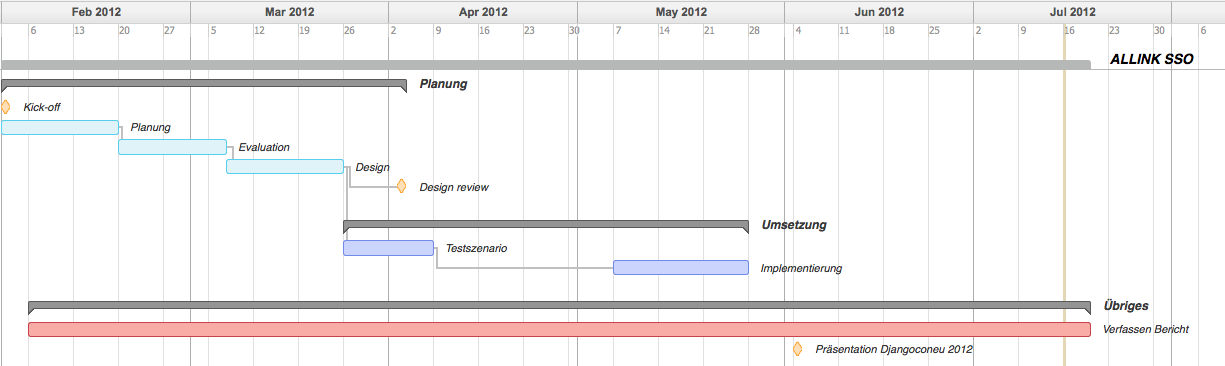
\includegraphics[width=21cm, angle=90]{include/zeitplan.png}
	\caption{Zeitplan}
	\label{fig:zeitplan}
\end{figure}

  
  \chapter{Analyse}
  \label{cha:Analyse}
  %!TEX root = ../index.tex
In diesem Kapitel wird die Situation wie sie vor dieser Arbeit war beschrieben. Es wurde bewusst darauf verzichtet Systeme und Gegebenheiten abzudecken, welche entweder kein Benutzermanagement aufweisen oder nicht von einem grossen Teil der Mitarbeiter eingesetzt werden.

\section{Systeme mit Benutzermanagement}
\label{sec:Systeme mit Benutzermanagement}

\subsection{Google-Apps}
\label{subs:Google-Apps}
Allink verwendet aus Google-Apps folgende Tools. 
\begin{itemize}
	\item Google Mail 
	\item Google Calendar 
	\item Google Sites 
	\item Google Docs 
	\item Google Analytics 
\end{itemize}

\subsection{Basecamp}
\label{subs:Basecamp}
Mit Basecamp werden Milestones und Todo-Listen für sämtliche Projekte verwaltet. Zudem werden sämtliche Arbeitsaufwände darin erfasst um am Ende eines Projekts einen Überblick über alle Arbeitsleistungen zu haben.

\subsection{Mac OS X Server}
\label{subs:Mac OS X Server}

\section{Mitarbeiter}
\label{sec:Mitarbeiter}
Um herauszufinden welche Benutzerdaten die Mitarbeiter kennen und welche Systeme sie nur verwenden können da das Passwort gespeichert wurde, wurde mit einer Umfrage der Sachverhalt erörtert.

\begin{tabular}
	{|l | c|} \hline System & Anzahl\\
	\hline Google-Apps & 10\\
	\hline Basecamp & 5\\
	\hline Mac OS X Server & 4\\
	\hline 
\end{tabular}

\section{Login Prozess}
\label{sec:Login Prozess}

\begin{figure}[H]  
		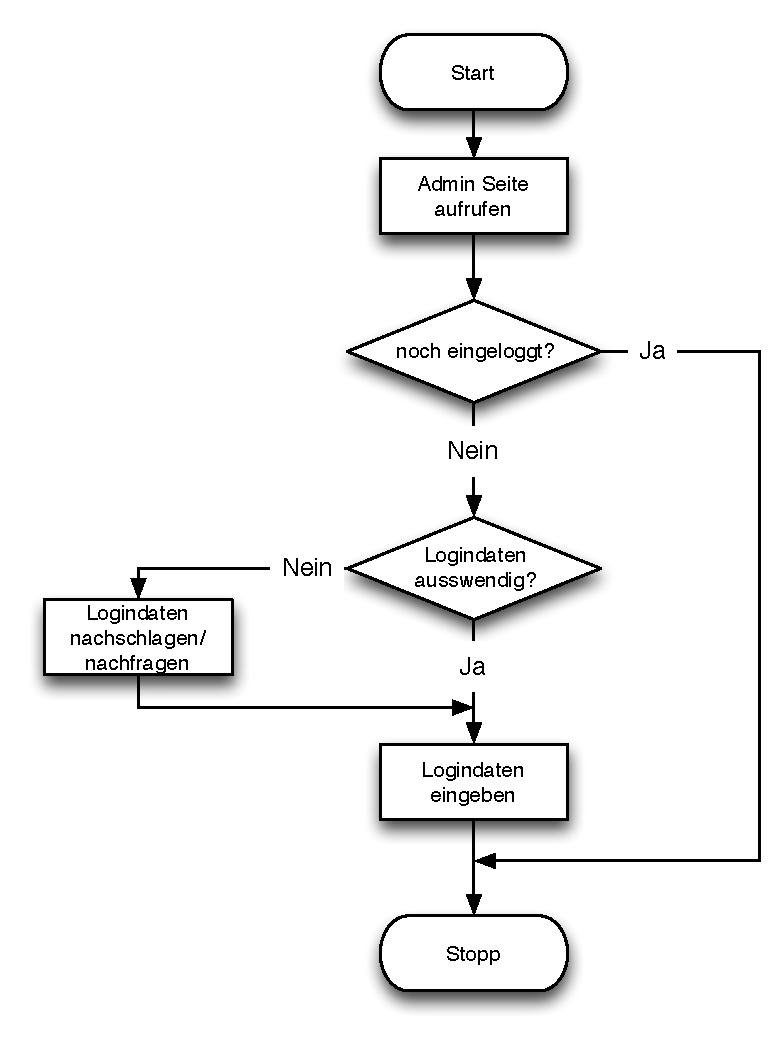
\includegraphics[width=0.70\textwidth]{include/login_before.pdf}
		\caption{Login Prozess vor dieser Arbeit}
		\label{fig:login-before}
\end{figure}

  
  \chapter{Anforderungen}
  \label{cha:Anforderungen}
  %!TEX root = ../index.tex
Die Anforderungen an eine Single-sign-On Lösung wurden bereits lange vor dieser Arbeit durch die technische Leitung der allink festgelegt. In diesen Anforderungen wird unter Benutzer ein Mitarbeiter der allink verstanden und unter Administrator ein Mitglied der technischen Leitung.

\section{Funktionale Anforderungen}
\label{sec:funktionale_anforderungen}
Die Single-sign-On Lösung sollte mindestens folgende Funktionalitäten erfüllen:
\begin{enumerate}
  \item Ein Benutzer kann sich mit seinen globalen Login-Daten an sämtlichen Webapplikationen der allink anmelden für die er berechtigt ist.
  \item Grundsätzlich sind alle Benutzer berechtigt sich an allen Webapplikationen anzumelden. Dies kann für einzelne Applikationen weiter eingeschränkt werden.
  \item Lokale Benutzerkonten, welche mit einem eigenen Passwort funktionieren, werden nur noch für die Kunden von allink verwendet.
  \item Ein neuer Benutzer kann an einem zentralen System erfasst werden, er hat sofort die Rechte für alle Webapplikationen welche keine besonderen Beschränkungen haben.
  \item Ein Benutzer kann zentral gesperrt werden. Danach ist es ihm nicht mehr möglich sich anzumelden. Bestehende Sitzungen werden nicht abgebrochen.
\end{enumerate}

\section{Technische Anforderungen}
\label{sec:technische_anforderungen}
Da diese SSO-Lösung für sehr viele Projekte eingesetzt werden soll, ist es wichtig, dass der nötige Aufwand um dies in einzelne Projekte zu integrieren möglichst klein gehalten wird.
  
  \chapter{Evaluation}
  \label{cha:Evaluation}
  %!TEX root = ../index.tex
Anwendungen welche mit externen Systemen kommunizieren, müssen auf einem Standard aufbauen welcher auch zukünftig noch unterstützt wird. Darum wurden zuerst die verschiedenen Standards betrachtet und danach mittels einer Nutzwert-Analyse ein System ausgewählt. Ein wichtiger Punkt für die Wahl eines Standards ist, dass die Integration in ein bestehendes Projekt möglichst einfach mit wenig Konfigurationsaufwand erreicht werden kann.

\section{Wahl eines Systems}
\label{sec:Wahl eines Systems}
Es gibt diverse Standards mit welchen man einen Benutzer identifizieren kann. Jedoch sind nicht alle davon für Webapplikationen geeignet. Um die Übersicht zu wahren wird hier nur auf zwei Typische Web Standards eingegangen. Damit auch eine Authentifizierung über Mac OS X Server erreicht werden könnte, wird zusätzlich noch kurz auf LDAP eingegangen.

\subsubsection{OpenID}
\label{ssub:OpenID}
Der offene Standard Openid wird von der OpenID
Foundation\footnote{\url{http://openid.net/foundation/}}, welche dafür gegründet wurde Marketing zu betreiben und die Rechte an der Marke OpenID zu wahren, gepflegt. Der Standard wurde dafür entwickelt, um es einem Benutzer welcher über eine OpenID verfügt zu ermöglichen sich an Webseiten welche OpenID unterstützen anzumelden ohne dass er sich einen neuen Benutzername und ein neues Passwort ausdenken muss. Das System welches die OpenID zur Verfügung stellt wird dabei \gls{OpenID-Provider} und die Webseiten an der sich der Benutzer anmeldet \glspl{OpenID-Relying-Party} genannt.

OpenID ist weit verbreitet und wird von vielen grösseren Webportalen unterstützt. Normalerweise erhält die \gls{OpenID-Relying-Party} nach dem ein Benutzer über OpenID eingeloggt hat, einen Identifier in form einer URL. Mit der attribute exchange Erweiterung lassen sich weitere Informationen über den Benutzer vom \gls{OpenID-Provider} beziehen.

\subsubsection{OAuth}
\label{ssub:OAuth}
Auch OAuth\footnote{\url{http://oauth.net}} ist ein offener Standard und ist zur Zeit in der Version 1.0 im RFC 5849\cite{rfc5849} aktuell. Jedoch verwenden die meisten Dienste heute schon OAuth 2.0 welches als Working Draft\footnote{\url{http://tools.ietf.org/html/draft-ietf-oauth-v2-26}} verfügbar ist. OAuth ist nicht für Authentifizierung gebaut sondern für Autorisierung. Es ermöglicht einem Benutzers einer Webapplikation die Vergabe von Rechten an einen weiteren Dienst, damit dieser bei der ersten Webapplikation API Funktionen aufrufen kann welche er ohne das Einverständnis des Benutzers keinen Zugriff hätte. Es lässt sich mit OAuth eine Pseudo-Authentifizierung durchführen, welche darauf beruht, dass nur der Benutzer diese Rechte erteilen kann. Dieses System wird von Facebook für die ``Login with Facebook'' verwendet.

\subsubsection{LDAP}
\label{ssub:LDAP}
Obwohl es unüblich ist für Webapplikationen LDAP\cite{rfc4511} zu verwenden, wurde diese Variante ebenfalls geprüft, da dies der einzige praktikable Weg wäre um eine Single-Sign-On Lösung mit einem Mac OS X Server als Kontenverwaltungsdienst zu erstellen.

\section{Nutzwert-Analyse}
\label{sec:Nutzwert-Analyse}
Da mehrere Systeme in der allink vorhanden sind welche sich für ein zentrales Login eignen, wurde eine Nutzwert-Analyse durchgeführt um die einzelnen Systeme miteinander zu vergleichen. Dabei wurde vor allem Wert darauf gelegt, dass nicht noch ein Login von den Mitarbeitern gemerkt werden muss.

\subsection{Gewichtung}
\label{sub:Gewichtung}
Die Gewichtung der einzelnen Punkte wurde in Zusammenarbeit mit der Allink Geschäftsleitung entwickelt. Jedoch war zu diesem Zeitpunkt noch nicht bekannt, welches System bei welchem Punkt seine Stärken ausspielen kann. Die so festgelegte Gewichtung kann ist Abbildung~\ref{fig:nutzwertanalyse gewichtung} zu sehen.

\begin{figure}[H]
    \centering 
		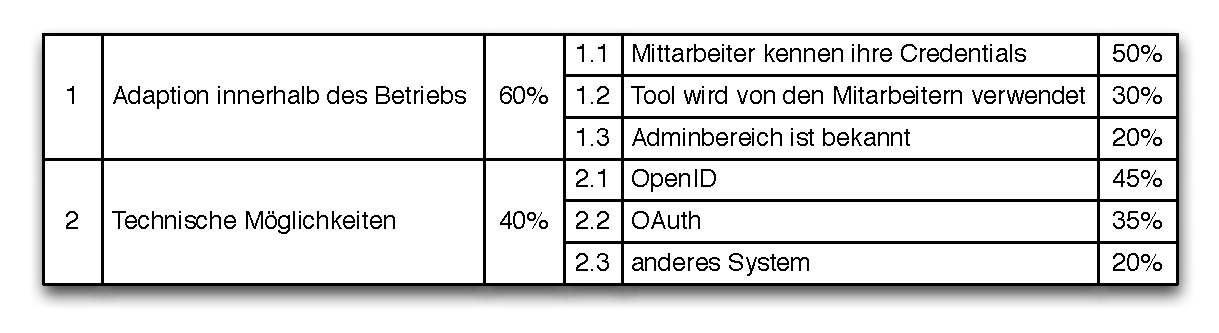
\includegraphics[width=1\textwidth]{include/nutzwertanalyse1.pdf}
		\caption{Gewichtung der einzelnen Faktoren}
		\label{fig:nutzwertanalyse gewichtung}
\end{figure}

\subsection{Bewertung}
\label{sub:Bewertung}
Die Systeme welche in der Analyse beschrieben wurden, wurden gemäss der in der Gewichtung genannten Punkte bewertet. Jeder Bewertungspunkt wurde nach der Skala in Tabelle~\ref{tab:nutzwertanalyse skala} bewertet. Nachfolgend wird auf die einzelnen Punkte eingegangen.

\begin{table}[h]
    \centering
        \begin{tabular}{|c|l|}
        \hline
        0 & Punkt nicht erfüllt\\
        \hline
        1 & Punkt ungenügend erfüllt\\
        \hline
        2 & Punkt genügend erfüllt\\
        \hline
        3 & Punkt erfüllt\\
        \hline
        4 & Punkt mehr als erfüllt\\
        \hline
        \end{tabular}
		\caption{Skala für die Punktevergabe}
		\label{tab:nutzwertanalyse skala}
\end{table}


\subsubsection{Mitarbeiter kennen ihre Credentials}
\label{ssub:Mitarbeiter kennen ihre Credentials}
Da das System den Mitarbeitern die Arbeit erleichtern soll wurde hier anhand der Umfrage welche unter Kapitel~\ref{sec:Mitarbeiter} erwähnt wurde verteilt.

\begin{tabular}{lc}
Google Apps & 3\\
Basecamp & 2\\
Mac OS X Server & 1\\
\end{tabular}

\subsubsection{Tool wird von den Mitarbeitern verwendet}
\label{ssub:Tool wird von den Mitarbeitern verwendet}
Unter diesem Punkt wurde beurteilt von wie vielen Mitarbeitern das geprüfte System bereits im Arbeitsalltag eingesetzt wird.
\paragraph{Google Apps}
\label{par:1.2Google Apps}
wird zur Zeit von allen Mitarbeitern verwendet, da darüber die E-Mail Dienste laufen. Zudem verwendet die IT und die Geschäftsleitung Google Docs und Google Sites.
\paragraph{Basecamp}
\label{par:1.2Basecamp}
wird vor allem von der Projektleitung verwendet, der Rest der Mitarbeiter verwendet Basecamp vor allemfür die Zeiterfassung, welche aber über ein Widget
geschieht und so nicht viel mit Basecamp zu tun hat.
\paragraph{Mac OS X Server}
\label{par:1.2Mac OS X Server}
wird von allen Mitarbeitern für den Austausch von Dateien und für das Backup verwendet. Jedoch sind sich die meisten Mitarbeiter nicht bewusst wo sie dieses System verwenden, da sie sich nie anmelden müssen.

\begin{tabular}{lc}
Google Apps & 4\\
Basecamp & 2\\
Mac OS X Server & 2\\
\end{tabular}

\subsubsection{Adminbereich ist bekannt}
\label{ssub:Adminbereich ist bekannt}
Da man für jeden neuen Mitarbeiter einen Account einrichten muss, und falls ein Mittarbeiter die Allink verlässt diesen Account wieder sperren muss, muss zumindest die Geschäftsleitung vertraut sein mit den entsprechenden Tools.
\paragraph{Google Apps}
\label{par:1.3Google Apps}
wird von der Informatik Leitung regelmässig verwendet. Daneben wird regelmässig Google Apps für Kunden eingerichtet und jeder Informatiker kennt sich im Administrationsbereich aus. Zudem sollte auch die gesamte Geschäftsleitung über Grundkenntnisse verfügen.
\paragraph{Basecamp}
\label{par:1.3Basecamp}
wird vor allem von der Projektleitung verwaltet. Jedoch ist das Erstellen eines neuen Mitarbeiters jeweils Aufgabe der Informatik Leitung.
\paragraph{Mac OS X Server}
\label{par:1.3Mac OS X Server}
wird nur von der Informatik Leitung konfiguriert und wird sonnst nicht verwendet.

\begin{tabular}{lc}
Google Apps & 4\\
Basecamp & 2\\
Mac OS X Server & 1\\
\end{tabular}

\subsubsection{OpenID}
\label{ssub:Bewertung OpenID}
OpenID ist die erste Wahl, da es in Python schon unterstützt wird und es dafür gedacht ist sich als Benutzer an einem System anzumelden.
\paragraph{Google Apps}
\label{par:2.1Google Apps}
unterstützt OpenID und wird auch auf der Webseite der OpenID Foundation gelistet.
\paragraph{Basecamp}
\label{par:2.1Basecamp}
unterstützte früher OpenID hat jedoch die Unterstützung am 1. Mai 2011 \footnote{\url{http://productblogarchive.37signals.com/products/2011/01/well-be-retiring-our-support-of-openid-on-may-1.html}} eingestellt.
\paragraph{Mac OS X Server}
\label{par:2.1Mac OS X Server}
unterstützt ohne zusätzliche Software kein OpenID.

\begin{tabular}{lc}
Google Apps & 3\\
Basecamp & 0\\
Mac OS X Server & 1\\
\end{tabular}

\subsubsection{OAuth}
\label{ssub:Bewertung OAuth}
Obwohl OAuth eigentlich nicht als authentifizierungs Protokoll gedacht ist. Kann es dafür verwendet werden indem man vom Provider die entsprechenden Daten bezieht. Dies ist jedoch zweite Wahl falls sich keine Möglichkeit bietet OpenID zu verwenden.
\paragraph{Google Apps}
\label{par:2.2Google Apps}
lässt über OAuth Zugriff auf Benutzerdaten und Schnittstellen zu.
\paragraph{Basecamp}
\label{par:2.2Basecamp}
lässt über OAuth Zugriff auf die gesamte API zu.
\paragraph{Mac OS X Server}
\label{par:2.2Mac OS X Server}
unterstützt kein OAuth.

\begin{tabular}{lc}
Google Apps & 3\\
Basecamp & 3\\
Mac OS X Server & 0\\
\end{tabular}

\subsubsection{anderes System}
\label{ssub:anderes System}
Um für den Fall, dass keines unserer Systeme geeignet ist um einen Benutzer mit OpenID oder OAuth zu authentifizieren, eine weitere Möglichkeit zu haben, wurde auch überprüft was unsere Systeme für weitere Möglichkeiten bieten.
\paragraph{Google Apps}
\label{par:2.3Google Apps}
bietet neben den schon erwähnten Möglichkeiten noch Unterstützung für SAML\footnote{\url{http://www.oasis-open.org/committees/tc_home.php?wg_abbrev=security}} jedoch zur Zeit nur um Benutzer von Google Diensten über ein Drittsystem zu Authentifizieren.
\paragraph{Basecamp}
\label{par:2.3Basecamp}
bietet keine weitere Möglichkeiten an.
\paragraph{Mac OS X Server}
\label{par:2.3Mac OS X Server}
hat standardmässig einen LDAP Dienst integriert. Darüber könnte man die nötige Authentifizierung und Autorisierung tätigen.

\begin{tabular}{lc}
Google Apps & 1\\
Basecamp & 0\\
Mac OS X Server & 3\\
\end{tabular}

\section{Auswertung}
\label{sec:Auswertung}
Wenn man die obigen Bewertungen gewichtet und summiert zeit sich ein klarer Sieger. Dies lässt sich dadurch erklären, dass Google die eigene Platform bewusst mit den nötigen Schnittstellen ausrüstet, weil es für Google Apps mittlerweile sogar einen Marktplatz für Zusatztools gibt.

\begin{table}[h!]
  \centering
  \begin{tabular}{|l|lr|lr|lr|lr|lr|lr|r|}
  \hline
  System & 1.1 & 0.3 & 1.2 & 0.18 & 1.3 & 0.12 & 2.1 & 0.18 & 2.2 & 0.14 & 2.3 & 0.08 & Total\\
  \hline
  Google Apps & 3 & 0.9 & 4 & 0.72 & 4 & 0.48 & 3 & 0.54 & 3 & 0.42 & 1 & 0.08 & 3.14\\
  \hline
  Basecamp & 2 & 0.6 & 2 & 0.36 & 2 & 0.24 & 0 & 0 & 3 & 0.42 & 0 & 0 & 1.62\\
  \hline
  Mac OS X Server & 1 & 0.3 & 2 & 0.36 & 1 & 0.12 & 1 & 0.18 & 0 & 0 & 3 & 0.24 & 1.2\\
  \hline
  \end{tabular}
  \caption{Auswertung der Nutzwertanalyse}
  \label{tab:auswertung_nutzwertanalyse}
\end{table}
  
  \chapter{OpenID}
  \label{cha:OpenID}
  %!TEX root = ../index.tex
Da die Wahl des zu verwendenden Protokolls auf OpenID fällt, wird an dieser Stelle die Funktionsweise von OpenID erklärt. Es ist nicht Bestandteil dieser Arbeit das OpenID Protokoll in Python zu implementieren, da dazu bereits eine Library existiert welche auch gewartet wird. Ryan Boyd von Google empfiehlt in einem Talk ausdrücklich davon abzusehen OpenID selber zu implementieren \cite[0:16:08]{googleioopenid}.

\section{Übersicht}
\label{sec:übersicht}
OpenID wurde entwickelt damit sich Benutzer an fremden Webseiten anmelden können, ohne dass sie ein neues Passwort kreieren müssen. OpenID ermöglicht es Benutzern eines \glsdisp{OpenID-Provider}{OpenID-Providers} sich an Webseiten welche als \gls{OpenID-Relying-Party} fungieren anzumelden. 

\section{Ablauf}
\label{sec:ablauf}
Abbildung~\ref{fig:openid_ablauf} zeigt den Ablauf der Authentisierung über OpenID. Es handelt sich hierbei um den einfachsten Ablauf. Es gibt noch weitere Abläufe, in denen zum Beispiel der Provider und die Relying-Party ein Shared Secret mittels Diffie Hellman\cite{rfc2631} vereinbaren, um damit die OpenID-Response mit einem HMAC\cite{rfc2104} zu versehen. Damit sind die Schritte 9 und 10 nicht mehr nötig, da nach dem Schritt 8 die Relying-Party bereits sicherstellen kann, dass die Response nicht verändert wurde und vom Provider stammt.
\begin{figure}[H]
  \centering
	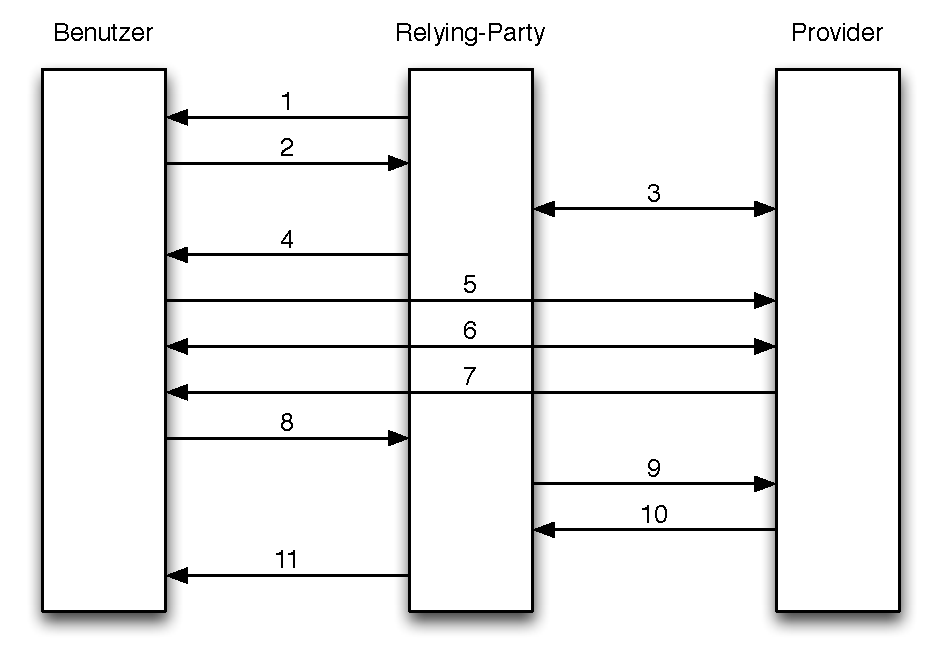
\includegraphics[width=0.9\textwidth]{include/openid1.pdf}
	\caption{OpenID Ablauf}
	\label{fig:openid_ablauf}
\end{figure}

\begin{enumerate}
  \item Relying-Party fordert den Benutzer auf sich anzumelden
  \item der Benutzer teilt der Relying-Party mit welcher Provider er verwenden möchte
  \item die Relying-Party führt eine Discovery durch um den Provider zu finden
  \item die Relying-Party übergibt dem Benutzer einen OpenID-Request
  \item der OpenID-Request wird vom Benutzer welcher weitergeleitet wird an den Provider geliefert
  \item falls nötig fordert der Provider den Benutzer auf sich anzumelden
  \item der Provider leitet den Benutzer mit der OpenID-Response an die Relying-Party weiter
  \item der Benutzer übergibt der Relying-Party die OpenID-Response
  \item die Relying-Party sendet dem Provider die OpenID-Response zur Bestätigung
  \item der Provider bestätigt der Relying-Party, dass die OpenID-Response von ihr verfasst wurde
  \item die Relying-Party leitet den Benutzer weiter auf eine Welcome-Seite
\end{enumerate}

\section{Sicherheit}
\label{sec:sicherheit}
Die Sicherheit von OpenID beruht vor allem auf dem Vertrauen in den OpenID-Provider. Da sich diese Arbeit darauf verlässt, dass die E-Mail-Adresse, welche vom OpenID-Provider geliefert wird, stimmt wurde auf die Schritte 1-3 aus Abbildung~\ref{fig:openid_ablauf} verzichtet und stattdessen ein OpenID-Provider in der Konfiguration hinterlegt.

\section{Erweiterungen}
\label{sec:erweiterungen}
Um über OpenID an die E-Mail-Adresse eines Benutzers zu gelangen, können zwei verschiedene Erweiterungen verwendet werden. Dies sind Simple Registration\cite{openid/sreg1.0} und Attribute Exchange\cite{openid/ax1.0}. Falls vorhanden wird Attribute Exchange vorgezogen, da Simple Registration einst als Minimalansatz entwickelt wurde und Attribute Exchange um einiges umfangreicher ist. 

  \chapter{Design}
  \label{cha:Design}
  %!TEX root = ../index.tex
\section{Entscheidungen}
\label{sec:Entscheidungen}

\subsection{Zu verwendendes System}
\label{sub:Zu verwendendes System}
Aus der Evaluation geht hervor, dass eine Anbindung an die OpenID Dienste von Google wohl am meisten Sinn macht. Google Apps ist ein fester Bestandteil der Arbeitsmittel jedes Mitarbeiters der Allink.

\subsection{Anmelde-Mechanismus}
\label{sub:Anmelde-Mechanismus}
Da in den meisten Fällen keine granulare Unterteilung der Benutzerrechte jedes einzelnen Mitarbeiters nötig ist. Da es viel mehr darum geht jedem Mitarbeiter von Allink Zugriff zu den Admin-Bereichen sämtlicher Webapplikationen zu gewähren und beim Enden dessen Arbeitsverhältnis diese Rechte wieder zu entziehen. Wird wie bisher für jede Webapplikation ein Benutzer mit vollen Administrator-Rechten erstellt. Bei erfolgreichem Anmelden über Google Apps ist der Mitarbeiter danach im Admin-Bereich mit diesem Benutzer angemeldet. Der Mitarbeiter bleibt danach für die Dauer seiner Session angemeldet.

\subsection{Wahl eines OpenID Providers}
\label{sub:Wahl eines OpenID Providers}
Da die Applikation um zu funktionieren nur einen OpenID Provider benötigt. Ist sie zumindest Theoretisch mit jedem beliebigen OpenID Provider verwendbar. Da wir die Mitarbeiter mit Hilfe der vom OpenID Provider verlangten E-Mail-Adresse identifizieren, und ein OpenID Provider diese E-Mail-Adresse fälschen könnte, kann der OpenID Provider nicht während des Login-Prozesses gewählt werden. Der Provider muss in den Einstellungen der Webapplikation hinterlegt werden. Falls jedoch kein Provider hinterlegt wurde, wird das Portal von Google als Standard verwendet.

\subsection{Abhängigkeiten}
\label{sub:Abhängigkeiten}
Da die zu erstellende Applikation in bestehende Projekte integriert werden soll, ist es wichtig die externen Abhängigkeiten so gering wie möglich zu gestalten. So wird nur für die Implementation von OpenID auf eine Bibliothek zurückgegriffen.

\subsubsection{Python OpenID}
\label{ssub:Python OpenID}
Da die korrekte Implementation von OpenID wichtig ist um die Sicherheit zu gewährleisten, ist es nicht ratsam OpenID ohne eine Library zu verwenden. In Python existiert zur Zeit nur eine Implementation von OpenID welche auch weiter entwickelt wird. Diese Library nennt sich python-openid und ist über den Python-Packet-Index\footnote{\url{http://pypi.python.org/pypi/python-openid/}} installierbar. Weiterentwickelt wird pyton-openid über das zugehörige Github Repository\footnote{\url{https://github.com/openid/python-openid}}.

\subsubsection{Django}
\label{ssub:Django}
Da ein Paket für das Django Webframework erstellt werden soll gehört Django auch zu den Abhängigkeiten. Um `Class Based Views' verwenden zu können benötigt man mindestens Version 1.3, welche zum Zeitpunkt dieser Arbeit bereits nicht mehr die aktuellste Version ist.

  
  \chapter{Tests}
  \label{cha:Tests}
  %!TEX root = ../index.tex
Da ein Single-Sign-On System aus Mindestens zwei Systemen besteht und in diesem Fall das eine bestehend ist, wird darauf verzichtet automatisierte Integrationstests zu erstellen. Stattdessen werden die wichtigsten Vorgänge mit Manuellen Testverfahren getestet.

\section{Ausgangslage}
\label{sec:TestingAusgangslage}
Um die Reproduzierbarkeit dieser Tests zu gewährleisten, müssen vor Beginn folgende Schritte getätigt werden.

\begin{itemize}
    \item Das Cache des Browsers muss geleert werden.
    \item Es darf keine offene Google-Apps Sitzung bestehen. Falls ein Benutzer
          angemeldet ist, muss dieser Abgemeldet werden.
    \item Die Datenbank des Testsystems muss neu Erstellt werden.
    \item Sämtliche Cookies welche zum Testsystem gehören müssen gelöscht
          werden.
    \item Ein Testbenutzer ist in Google-Apps erstellt und aktiv.
\end{itemize}


\begin{tabular}{p{7cm} p{7cm}}
Aktion & Erwartetes Resultat\\
\hline
Drücken des ``Login mit OpenID'' Buttons im Admin & Der Browser wechselt zum Google Login\\
Eingeben der Benutzerdaten & Django Admin Startseite wird angezeigt und der zugewiesene Benutzer ist angemeldet\\
Löschen der Session des Testsystems und neu laden der Seite & Die Login-Seite erscheint\\
Sperren des Benutzers in Google-Apps mit einem anderen Browser & Kein Resultat erwartet\\
Drücken des ``Login mit OpenID'' Buttons im Admin & Der Browser wechselt zum Google Login\\
Eingeben der Benutzerdaten & Benutzer darf sich nicht anmelden können\\
\end{tabular}

  
  \chapter{Umsetzung}
  \label{cha:Umsetzung}
  %!TEX root = ../index.tex
\section{Opensource}
\label{sec:opensource}
Da es der Philosophie von allink gehört, entwickelte Tools welche auch für andere Agenturen und Webentwickler von Nutzen sein könnten zu veröffentlichen. Dies aus zwei verschiedenen Gründen auf welche hier kurz eingegangen wird.

\paragraph{Steigerung der Reputation}
\label{par:steigerung_der_reputation}
Um allink für potentielle Mitarbeiter im Webbereich attraktiver zu machen.
\paragraph{Chance auf Mitarbeit Dritter}
\label{par:chance_auf_mitarbeit_dritter}
Wenn ein von allink veröffentlichtes Tool von Dritten genutzt wird, besteht die Chance, dass diese das Tool weiterentwickeln oder bestehende Fehler beheben.

\subsection{Lizenz}
\label{sub:lizenz}
Um ein Tool für Dritte nutzbar zu machen und um zu gewährleisten, dass diese auch den Quellcode des Tools ändern dürfen, muss das ganze Tool unter einer Softwarelizenz, welche dies gestattet, veröffentlicht werden. Die drei Klausel BSD Lizenz\footnote{\url{http://www.opensource.org/licenses/BSD-3-Clause}} lässt dem Lizenznehmer genügend Freiheiten um den Quellcode zu verwenden wo er will. Das Framework Django ist ebenfalls unter der drei Klausel BSD Lizenz veröffentlich worden.

\subsection{Versionsverwaltung}
\label{sub:versionsverwaltung}
Es wurde \glossary{Git} für die Versionierung verwendet da dies dem Standard der allink gehört. Es wurde ein zentrales Repository\footnote{\url{https://github.com/frog32/django-admin-sso}} auf Github eingerichtet um den Quellcode zu veröffentlichen.

\section{Python Paket}
\label{sec:Python Paket}
Es gibt zwei grundsätzlich verschiedene Distributionsarten für Python Pakete. ``Source'' Distributionen sind Archive mit den benötigten Python Dateien zusammen mit einem Setup-Script. ``Builded'' Distributionen hingegen sind für ein bestimmtes System gebaut und lassen sich typischerweise über den Systemeigenen Packet Manager oder im Fall von Windows, über ein Installationsprogramm installieren. Python Pakete welche für den Gebrauch in Webapplikationen konzipiert sind, sind normalerweise als ``Source''-Distribution erhältlich. Diese ``Source''-Distributionen werden dann mit easy\_install\footnote{\url{http://packages.python.org/distribute/easy_install.html}} oder pip\footnote{\url{http://www.pip-installer.org/}} Installiert. Alternativ können ``Source''-Distributionen auch durch simples Entpacken und Ausführen des Installations-Skripts installiert werden. Da ``django-admin-sso'' nur für die Verwendung in Webapplikationen vorgesehen ist, wird nur eine ``Source''-Distribution erstellt.

\subsection{Paketerstellung}
\label{sub:paketerstellung}
Ein Python-Paket wird durch verschiedene Dateien charakterisiert. Auf die für die Distribution verwendete Tateien wird in Tabelle~\ref{tab:paket_inhalt} eingegangen. Im Manifest wurden zusätzlich noch nicht existierende Dateien erwähnt welche für eine Übersetzung des Paketes in mehrere Sprachen verwendet werden.

\begin{table}[h]
  \centering
  \begin{tabular}{|l|l|p{7cm}|}
  \hline
  Dateiname & Zwingend & Inhalt\\
  \hline
  AUTHORS & Nein & eine Liste aller Authoren\\
  \hline
  LICENSE & Nein & die verwendete Softwarelizenz\\
  \hline
  MANIFEST.in & Nein & eine Liste von nicht Python Dateien welche berücksichtigt werden muss\\
  \hline
  setup.cfg & Nein & Einstellungen für Dokumentationstools\\
  \hline
  setup.py & Ja & Konfiguration des Installationsprogramms\\
  \hline
  \end{tabular}
  \label{tab:paket_inhalt}
  \caption{Dateien und ihre Funktion für eine Distribution}
\end{table}

\subsection{Registration}
\label{sub:registration}
Der ``Python Packet Index''\footnote{\url{http://pypi.python.org/}} bildet die zentrale Registrierungsstelle für alle Python Pakete. Es ist ratsam jedes Paket welches für den freien Gebrauch bestimmt ist in diesem Index zu registrieren.\footnote{\url{http://pypi.python.org/pypi/django-admin-sso/}}

Zusätzlich zum ``Python Packet Index'' wurde das Paket auch in den Index von ``Django Packages''\footnote{\url{http://www.djangopackages.com/packages/p/django-admin-sso/}} eingetragen. Diese Platform wird von vielen Django-Entwicklern verwendet um neue Pakete zu evaluieren.


  \chapter{Resultate}
  \label{cha:Resultate}
  %!TEX root = ../index.tex
Das sicher wichtigste Resultat dieser Arbeit bildet die funktionsfähige Applikation welche es ermöglicht sich mit einer OpenID an einem Administrationsbereich anzumelden. Diese Applikation wird bei jeder neuen Webseite eingesetzt und wurde zudem in den wichtigsten bestehenden Webseiten bereits eingebaut.

\section{Erfüllung der Anforderungen}
\label{sec:erfüllung_der_anforderungen}
Django-admin-sso erfüllt alle in Kapitel~\ref{sec:funktionale_anforderungen} definierten Anforderungen und lässt sich einfach in bestehende und neue Projekte integrieren. Die Installation des Paketes ist über den Python Packet Index und einem Python Paket-Management sehr einfach. Die technischen Anforderungen aus Kapitel~\ref{sec:technische_anforderungen} werden meines Erachtens gut erfüllt.

\section{Reaktionen}
\label{sec:reaktionen}
Am 4.Juni 2012 habe ich spontan das Projekt an der Djangoconeu 2012~\footnote{http://2012.djangocon.eu/} während eines Lightning Talks vorgestellt. Der Talk bestand im wesentlichen in einer während der Konferenz vorbereiteten live Demonstration. Nach dem Talk haben sich mehrere Personen bei mir gemeldet und mir erzählt, dass auch sie schon lange auf der Suche nach einer solchen Lösung waren.

Das Projekt hat zur Zeit~\footnote{Stand vom 16.Juli 2012} 15 Watchers auf Github und und bisher 4 Pull Requests mit kleineren Anpassungen. Das Paket hat bereits 396 Downloads über den Python Packet Index. Auf meine Anfrage ob sie django-admin-sso produktiv einsetzen bekam ich von Matthias Kestenholz und Marc Tamlyn folgende Antworten:

\paragraph{Matthias Kestenholz}
Programmierung \& Qualitätssicherung bei FEINHEIT GmbH
\begin{quote}
  Hi Marc

  Unfortunately we aren't using sso yet, but I'd very much like to.

  It certainly gave us a few good ideas how to solve the problem where
  former employees still have access to many websites just because they
  know the passwords we use. I think we should start using it on all
  sites except for a few special ones (not that I'd think of any
  projects in particular, but there are pages which have a different
  audience, especially webapps or plattforms).


  Thanks \\
  Matthias
\end{quote}

\paragraph{Marc Tamlyn}
Developer bei INCUNA LTD.
\begin{quote}
  Hi Marc,

  We have implemented admin-sso into our base project, and it is being used on all new applications. There may be some apps where we can't use it due to clients having odd requirements on security, but it is not enabled by default.

  Thanks for such a useful project!

  Marc
\end{quote}


  \chapter{Fazit}
  \label{cha:Fazit}
  %!TEX root = ../index.tex
Das Szenario, dass sich ehemalige Mitarbeiter an Passwörter erinnern und mit diesem Wissen versuchen der Agentur oder einem Kunden Schaden zuzufügen, hat sich bisher glücklicherweise nicht ergeben. Jedoch können wir nun mit einfachen Mitteln ehemaligen Mitarbeitern den Zugang zu  von uns betreuten Webseiten sperren. Auch wenn in der Praxis wahrscheinlich nie Probleme entstehen würden, lässt uns der Einsatz von django-admin-sso besser schlafen.

Diese Arbeit hat ihren Ursprung im Herbst 2011, als wir uns in der allink ein Zeitbudget von zwei Tagen reserviert hatten um alle Mitarbeiter über ein zentrales System zu autorisieren. Schnell hatte sich damals gezeigt, dass in den zwei Tagen keine praktikable Lösung erzielt werden konnte. Daraufhin entstand die Idee meine Semesterarbeit dem Thema zu widmen.

Ich konnte durch diese Arbeit an der Djangoconeu 2012 viele Kontakte zu Webentwicklern knüpfen, welche das gleiche Problem hatten wie wir. Von diesen setzen heute zumindest einige meine Applikation ein. Ich konnte zudem im Zuge der Arbeit meine Kenntnisse in diversen weniger oft verwendeten Gebieten auffrischen oder vertiefen. Zu diesen Gebieten gehören unter anderem das erstellen eines Python Paketes, erstellen von Dokumentationen mit LaTeX und das Anwenden von Projektplanungstools.
  
  \appendix  
  \listoffigures
  \listoftables
  \lstlistoflistings
  
  \glsaddall
  \printglossaries
  
  \nocite{*}
  \bibliographystyle{alphadin}
  \bibliography{cite}
\end{document}
